%
%  Chris Thoma
%
\documentclass[12pt,fullpage]{article}
\usepackage{fullpage}
\usepackage{psfrag}                                          % LaTeX graphics tool
\usepackage{pslatex}                                         % avoids the default cmr font
\usepackage{graphicx}                                        % graphics package 
\usepackage{epsfig}                                          % figures
\usepackage{hyperref}
\usepackage{color}

\begin{document}

\noindent
{\bf T distribution}  (from \color{blue}\url{http://www.math.wm.edu/~leemis/chart/UDR/UDR.html}\color{black})

\noindent
The shorthand $X \sim t(n)$ is used to indicate that the
random variable $X$ has the $t$ distribution with positive,
real-valued parameter $n$, known as the degrees of freedom.
In most applications, $n$ is a positive integer.
A $t$ random variable $X$ with $n$ degrees of freedom has
probability density function 
$$
f(x) = \frac{\Gamma((n+1)/2)(1 + x^2/n) ^ {(-(n+1)/2)}}
{\sqrt{n \kern 0.08 em \pi} \kern 0.08 em \Gamma \left( n/ 2 \right)}
\qquad \qquad -\infty < x < \infty.
$$
The $t$ distribution arises in hypothesis tests concerning the
comparison of (a) a sample mean to a standard, or (b)
the difference between two means.
The probability density function for $n=1$ (a special case of
the $t$ distribution known as the Cauchy distribution) and
$n=5$ is illustrated below.
{\begin{figure}[h!]
\begin{center}
\psfrag{lab1}{$n \kern -0.08 em = \kern -0.08 em 1$}
\psfrag{lab2}{$n \kern -0.08 em = \kern -0.08 em 5$}
\psfrag{labx}{$x$}
\psfrag{labf}{$f(x)$}
\includegraphics[width=3.2in]{TPlot.ps}
\end{center}
\end{figure}}\\
The cumulative distribution function on the support of $X$ is
$$
F(x) = P(X \le x) = \displaystyle \int_{-\infty} ^ {x}
\frac{\Gamma((n+1)/2) n ^ {n/2} (n + t ^ 2) ^ {\big((n-1)/2\big)}}{\sqrt{\pi}
\kern 0.08 em \Gamma \left( n/2 \right)} \ dt
\qquad \qquad -\infty < x < \infty.
$$
The survivor function on the support of $X$ is
$$
S(x) = P(X \ge x) = \displaystyle \int_{x} ^ {\infty}
\frac{\Gamma((n+1)/2) n ^ {n/2} (n + t ^ 2) ^ {\big((n-1)/2\big)}}{\sqrt{\pi}
\kern 0.08 em \Gamma \left( n/2 \right)} \ dt
\qquad \qquad -\infty < x < \infty.
$$

%The hazard function on the support of $X$ is
%$$
%h(x) = \frac{f(x)}{S(x)} = -\frac{n ^ {\frac{n} {2}} (n + x ^ 2) ^ {-(\frac{1} {2} -\frac{n} {2})} \Gamma(\frac{1}{2} + \frac{n}{2})} {\sqrt{\pi}\left(-1 + \displaystyle \int_{-\infty} ^ {x} \frac{\Gamma(\frac{1} {2} + \frac{n}{2}) n ^ {(\frac{n}{2})} (n + t ^ 2) ^ {-(\frac{1} {2} - \frac{n} {2})}}{\sqrt{\pi} \kern 0.08 em \Gamma \left(\frac{n}{2}\right)} \ dt \right) \Gamma(\frac{n}{2})} \qquad \qquad -\infty < x < \infty.
%$$
The hazard function and cumulative hazard function on the support of $X$ is mathematically intractable.\\
\\
The inverse distribution function of $X$ is mathematically intractable.\\
\\
The median of $X$ is $0$ because $f(x)$ is an even function.\\
\\
The moment generating function of $X$ is undefined, although various
moments exist for restricted values of the parameter $n$.\\
\\
The population mean, variance, skewness, and kurtosis of $X$ are
$$
E[X] = 0 \quad  {\rm for} \ n > 1, \qquad \qquad
V[X] = \frac{n}{n-2} \quad {\rm for} \ n > 2, \quad 
$$
$$
E\left[ \left( \frac{X - \mu}{\sigma} \right) ^ 3 \right] = 0 \quad  {\rm for} \ n > 3,\qquad \qquad
E\left[ \left( \frac{X - \mu}{\sigma} \right) ^ 4 \right] = \frac{3(n-2)}{n-4} \quad {\rm for} \  n > 4.\quad
$$
\noindent
{\bf APPL verification:}
The APPL statements
\begin{verbatim}
 X := TRV(n);
 CDF(X);
 SF(X);
 Mean(X);
 Variance(X);
 Skewness(X);
 Kurtosis(X);
\end{verbatim}
verify the cumulative distribution function, survivor function, hazard function,
population mean, variance, skewness, and kurtosis.

\end{document}
